\chapter{System Design and Implementation}

\section{Architectural Overview}

CitySense is structured as a three-layer system:

\begin{enumerate}[label=\arabic*.]
  \item a Flutter mobile client used by citizens to capture and submit pothole reports;
  \item a FastAPI backend responsible for validation, detection, persistence, and duplicate handling;
  \item a lightweight web dashboard that visualizes active reports and supports status management.
\end{enumerate}

The architectural goal is to keep the mobile workflow small and intuitive while delegating processing-heavy tasks to the backend. Image capture, permission handling, and map viewing remain on the client. Detection, spatial queries, and persistence remain on the server. This separation also keeps the core business logic centralized in one place, which simplifies both testing and thesis documentation.

\section{Mobile Application}

The mobile client is implemented in Flutter. The application is Android-first in the current version, but the codebase is organized so that API communication, location retrieval, and screen logic are separated into reusable services. The mobile interface contains two principal screens:

\begin{itemize}
  \item a \textbf{Report} screen that captures the image, fetches the current GPS location, submits the report, and displays submission feedback;
  \item a \textbf{Map} screen that displays open reports as markers and allows the user to inspect report metadata.
\end{itemize}

This structure is visible in the application interface shown in Figure~\ref{fig:app_interface}. The screen is intentionally simple because the main design objective is to minimize user friction. Instead of collecting a textual description from the user, the application sends the image and coordinates to the backend and displays the result returned by the detector.

\begin{figure}[htbp]
    \centering
    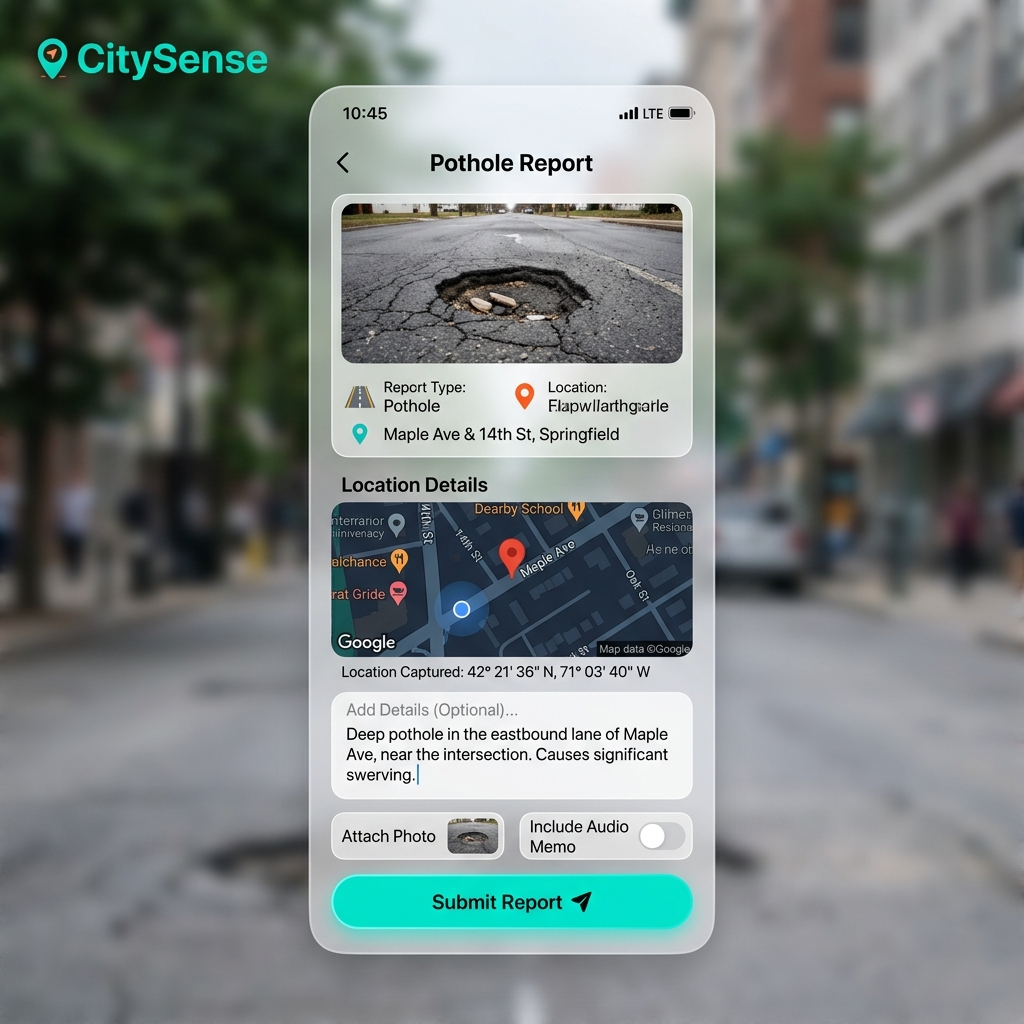
\includegraphics[width=0.45\textwidth]{figures/app_interface_pothole_1775200631079.png}
    \caption{CitySense mobile application interface for photo-based pothole reporting.}
    \label{fig:app_interface}
\end{figure}

\section{Backend Service}

The backend is implemented in Python with FastAPI. It exposes a small REST interface that matches the needs of the mobile client and the admin dashboard. The current API surface is summarized in Table~\ref{tab:api_endpoints}.

\begin{table}[htbp]
\centering
\begin{tabular}{>{\raggedright\arraybackslash}p{0.28\linewidth} >{\raggedright\arraybackslash}p{0.62\linewidth}}
\toprule
\textbf{Endpoint} & \textbf{Purpose} \\
\midrule
\texttt{GET /api/v1/health} & Returns runtime information such as detector mode, upload directory, and duplicate radius. \\
\texttt{POST /api/v1/reports} & Accepts a pothole image and geographic coordinates, runs detection, and either creates or merges a report. \\
\texttt{GET /api/v1/reports} & Returns report data for the mobile map and the admin dashboard. \\
\texttt{PATCH /api/v1/reports/\{id\}/status} & Updates a report from \texttt{OPEN} to \texttt{RESOLVED}. \\
\bottomrule
\end{tabular}
\caption{Public backend endpoints used by CitySense.}
\label{tab:api_endpoints}
\end{table}

The backend uses SQLAlchemy models to persist reports in PostgreSQL. Each report stores the issue type, detector confidence, latitude, longitude, geographic point, image path, status, upvote count, and timestamps. The system currently focuses on the \texttt{pothole} issue type because that keeps the label space explicit and consistent with the intended detector workflow.

\section{Duplicate Detection with PostGIS}

One of the most important implementation details is the duplicate merge strategy. A new report is not automatically inserted as a new row. Instead, the backend constructs a geographic point from the incoming latitude and longitude and compares it against open reports of the same issue type. The comparison is performed with \texttt{ST\_DWithin}, using a 10 meter threshold.

If a matching open report already exists, the new submission increments the upvote counter of the existing record. If no match is found, the backend creates a new report. This design keeps the map readable and makes the administrative view more useful, because repeat submissions become a signal of urgency rather than database noise.

\section{Detection Pipeline}

The detector layer is implemented as a dedicated backend service. In the intended thesis configuration, the backend loads a trained pothole checkpoint and accepts only pothole-like labels from the detector output. The implementation also includes a clearly marked \texttt{demo} detector mode that returns deterministic pothole responses for UI smoke testing when a trained checkpoint is not yet present. This decision keeps the rest of the stack testable without pretending that a generic detector is sufficient for pothole recognition.

Figure~\ref{fig:yolo_detection} shows a sample detection-style output used to illustrate the intended visual feedback of the YOLO pipeline. The repository also includes scripts for fine-tuning and evaluation so that a dedicated pothole checkpoint can be produced from an RDD2022-style dataset.

\begin{figure}[htbp]
    \centering
    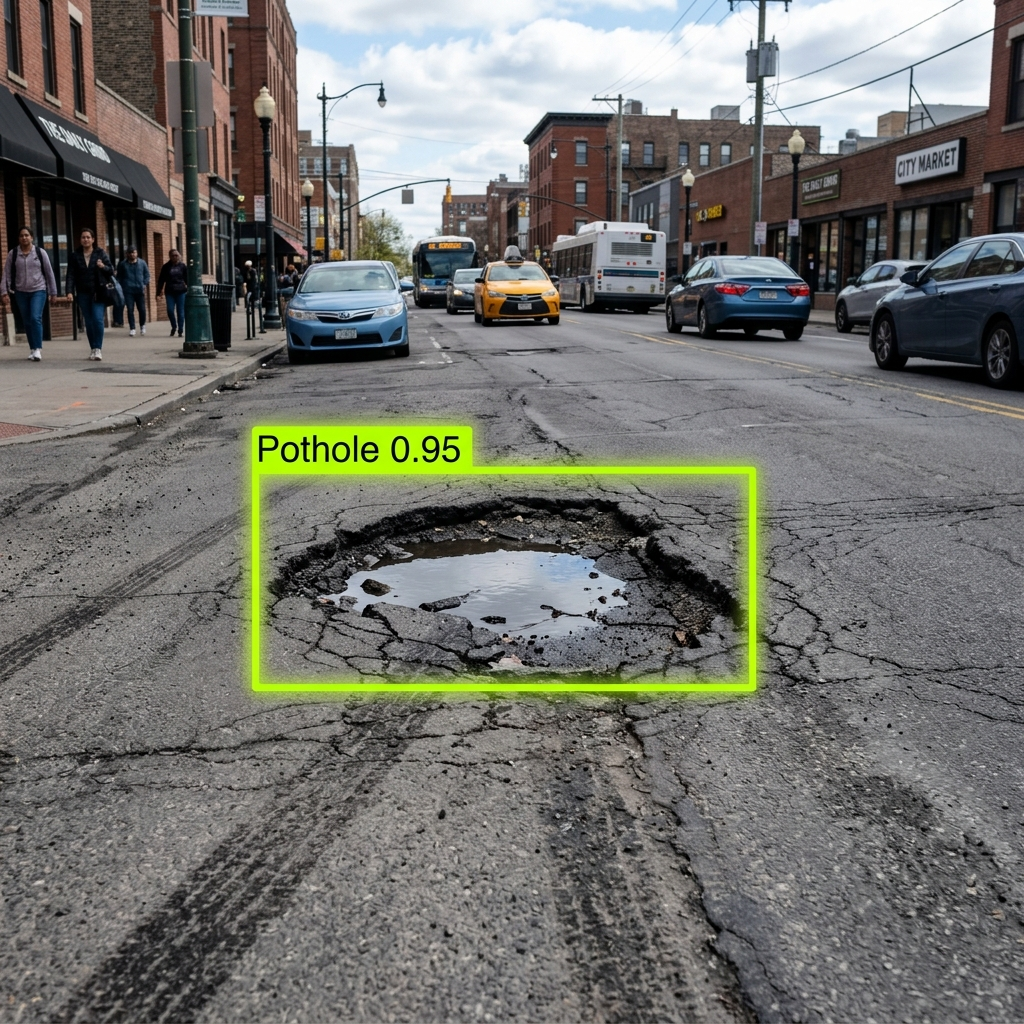
\includegraphics[width=0.78\textwidth]{figures/yolo_detection_demo_1775200664858.png}
    \caption{Illustrative detector output for the CitySense pothole-recognition pipeline.}
    \label{fig:yolo_detection}
\end{figure}

\section{Administrative Dashboard}

The administrator-facing interface is a lightweight web page built around Leaflet and OpenStreetMap tiles. It is intentionally separate from the mobile client because the administrative role requires a different view of the data: status filters, marker clustering by proximity, direct access to upvote counts, and the ability to mark a report as resolved.

Figure~\ref{fig:admin_dashboard} presents the dashboard concept used in the project. The current implementation shows report cards, a geographic map layer, report metadata, and a resolve action. This is enough to support the demonstration scenario of the thesis without overextending the scope into a full municipal operations platform.

\begin{figure}[htbp]
    \centering
    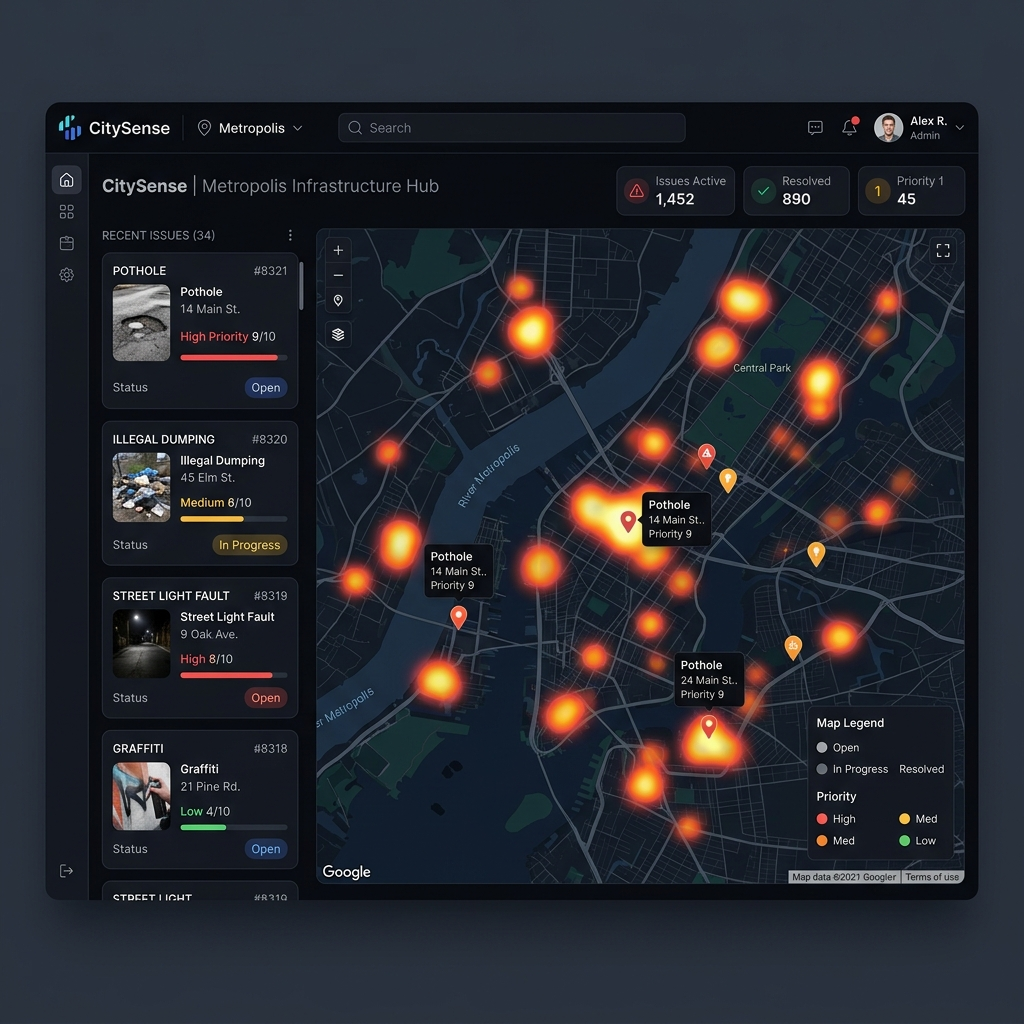
\includegraphics[width=0.85\textwidth]{figures/admin_dashboard_map_1775200648148.png}
    \caption{Administrative dashboard for viewing and resolving reported potholes.}
    \label{fig:admin_dashboard}
\end{figure}

\section{Monorepo Organization}

The final implementation is maintained as a monorepo with three main directories: backend, mobile client, and thesis source. This organization supports reproducibility in two ways. First, it keeps documentation synchronized with code evolution. Second, it makes setup instructions more coherent because the API, the app, and the thesis all live in one repository and can be versioned together.
